% This file was created with tikzplotlib v0.9.12.
\begin{figure}[h!]
\centering
% This file was created with tikzplotlib v0.9.12.
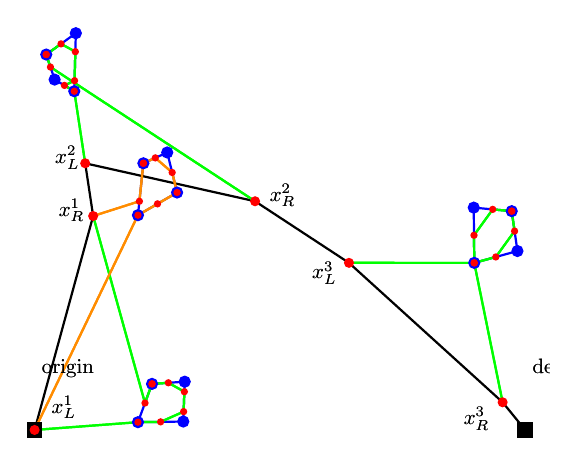
\begin{tikzpicture}

\definecolor{color0}{rgb}{1,0.549019607843137,0}

\begin{axis}[
hide x axis,
hide y axis,
scaled x ticks=manual:{}{\pgfmathparse{#1}},
scaled y ticks=manual:{}{\pgfmathparse{#1}},
tick align=outside,
x grid style={white!69.0196078431373!black},
xmajorticks=false,
xmin=-5, xmax=105,
xtick style={color=black},
xticklabels={},
y grid style={white!69.0196078431373!black},
ymajorticks=false,
ymin=-5, ymax=75,
ytick style={color=black},
yticklabels={}
]
\path [draw=blue, thick]
(axis cs:21.0696182692914,1.38670279952717)
--(axis cs:30.306045132353,1.50447958089156);

\path [draw=blue, thick]
(axis cs:21.0696182692914,1.38670279952717)
--(axis cs:23.9355243392435,8.22107815581281);

\path [draw=blue, thick]
(axis cs:30.306045132353,1.50447958089156)
--(axis cs:30.6007400849981,8.61180925900065);

\path [draw=blue, thick]
(axis cs:23.9355243392435,8.22107815581281)
--(axis cs:30.6007400849981,8.61180925900065);

\path [draw=blue, thick]
(axis cs:4.08370396767994,62.5193171258523)
--(axis cs:8.09069545603466,60.4417973648425);

\path [draw=blue, thick]
(axis cs:4.08370396767994,62.5193171258523)
--(axis cs:2.37426610997379,66.9905560181573);

\path [draw=blue, thick]
(axis cs:8.09069545603466,60.4417973648425)
--(axis cs:8.40433589338944,70.7975020391092);

\path [draw=blue, thick]
(axis cs:2.37426610997379,66.9905560181573)
--(axis cs:8.40433589338944,70.7975020391092);

\path [draw=blue, thick]
(axis cs:21.0664581490033,38.3255279820558)
--(axis cs:29.0472438012912,42.369596955967);

\path [draw=blue, thick]
(axis cs:21.0664581490033,38.3255279820558)
--(axis cs:22.1750046919912,47.5858849832036);

\path [draw=blue, thick]
(axis cs:29.0472438012912,42.369596955967)
--(axis cs:27.0356718607916,49.5164362980235);

\path [draw=blue, thick]
(axis cs:22.1750046919912,47.5858849832036)
--(axis cs:27.0356718607916,49.5164362980235);

\path [draw=blue, thick]
(axis cs:89.6170857784204,29.8130206242151)
--(axis cs:98.4204942730176,31.9280359170996);

\path [draw=blue, thick]
(axis cs:89.6170857784204,29.8130206242151)
--(axis cs:89.5168058385155,39.6742972814671);

\path [draw=blue, thick]
(axis cs:98.4204942730176,31.9280359170996)
--(axis cs:97.2556927544101,39.0446066906692);

\path [draw=blue, thick]
(axis cs:89.5168058385155,39.6742972814671)
--(axis cs:97.2556927544101,39.0446066906692);

\path [draw=black, thick]
(axis cs:0,0)
--(axis cs:0,0)
--(axis cs:11.9384375817266,38.1768740390765)
--(axis cs:10.3131414759248,47.5858849832036)
--(axis cs:44.9451427093311,40.8090894507933)
--(axis cs:64.0827735142413,29.8198845110857)
--(axis cs:95.4029040306271,4.93918065109767)
--(axis cs:100,0);
\path [draw=green, thick]
(axis cs:0,0)
--(axis cs:21.0696182692914,1.38670279952717)
--(axis cs:25.6878317008222,1.44559119020937)
--(axis cs:30.3792241725836,3.26938108252212)
--(axis cs:30.5265716489061,6.82304592157666)
--(axis cs:27.2681322121208,8.41644370740673)
--(axis cs:23.9355243392435,8.22107815581281)
--(axis cs:23.9355243392435,8.22107815581281)
--(axis cs:22.5025713042674,4.80389047767)
--(axis cs:11.9384375817266,38.1768740390765);
\path [draw=color0, thick]
(axis cs:0,0)
--(axis cs:21.0664581490033,38.3255279820558)
--(axis cs:25.0568509751472,40.3475624690114)
--(axis cs:29.0472438012912,42.369596955967)
--(axis cs:28.0414578310414,45.9430166269952)
--(axis cs:24.6053382763914,48.5511606406136)
--(axis cs:22.1750046919912,47.5858849832036)
--(axis cs:22.1750046919912,47.5858849832036)
--(axis cs:21.3637623976544,40.8090894507933)
--(axis cs:11.9384375817266,38.1768740390765);
\path [draw=green, thick]
(axis cs:0,0)
--(axis cs:21.0696182692914,1.38670279952717)
--(axis cs:25.6878317008222,1.44559119020937)
--(axis cs:30.3792241725836,3.26938108252212)
--(axis cs:30.5265716489061,6.82304592157666)
--(axis cs:27.2681322121208,8.41644370740673)
--(axis cs:23.9355243392435,8.22107815581281)
--(axis cs:23.9355243392435,8.22107815581281)
--(axis cs:22.5025713042674,4.80389047767)
--(axis cs:11.9384375817266,38.1768740390765);
\path [draw=color0, thick]
(axis cs:0,0)
--(axis cs:21.0664581490033,38.3255279820558)
--(axis cs:25.0568509751472,40.3475624690114)
--(axis cs:29.0472438012912,42.369596955967)
--(axis cs:28.0414578310414,45.9430166269952)
--(axis cs:24.6053382763914,48.5511606406136)
--(axis cs:22.1750046919912,47.5858849832036)
--(axis cs:22.1750046919912,47.5858849832036)
--(axis cs:21.3637623976544,40.8090894507933)
--(axis cs:11.9384375817266,38.1768740390765);
\path [draw=green, thick]
(axis cs:10.3131414759248,47.5858849832036)
--(axis cs:8.09069545603467,60.4417973648425)
--(axis cs:6.08719971185731,61.4805572453474)
--(axis cs:8.1475539671049,62.3191380350312)
--(axis cs:8.30437418578229,67.4969903721645)
--(axis cs:5.38930100168162,68.8940290286332)
--(axis cs:2.37426610997379,66.9905560181573)
--(axis cs:2.3742661099738,66.9905560181572)
--(axis cs:3.22898503882687,64.7549365720048)
--(axis cs:44.9451427093311,40.8090894507933);
\path [draw=green, thick]
(axis cs:10.3131414759248,47.5858849832036)
--(axis cs:8.09069545603467,60.4417973648425)
--(axis cs:6.08719971185731,61.4805572453474)
--(axis cs:8.1475539671049,62.3191380350312)
--(axis cs:8.30437418578229,67.4969903721645)
--(axis cs:5.38930100168162,68.8940290286332)
--(axis cs:2.37426610997379,66.9905560181573)
--(axis cs:2.3742661099738,66.9905560181572)
--(axis cs:3.22898503882687,64.7549365720048)
--(axis cs:44.9451427093311,40.8090894507933);
\path [draw=green, thick]
(axis cs:64.0827735142413,29.8198845110857)
--(axis cs:89.6170857784204,29.8130206242151)
--(axis cs:94.018790025719,30.8705282706573)
--(axis cs:97.8380935137139,35.4863213038844)
--(axis cs:97.2556927544101,39.0446066906692)
--(axis cs:97.25569275441,39.0446066906692)
--(axis cs:93.3862492964628,39.3594519860681)
--(axis cs:89.5669458084679,34.7436589528409)
--(axis cs:89.6170857784204,29.8130206242149)
--(axis cs:95.4029040306271,4.93918065109767);
\path [draw=green, thick]
(axis cs:64.0827735142413,29.8198845110857)
--(axis cs:89.6170857784204,29.8130206242151)
--(axis cs:94.018790025719,30.8705282706573)
--(axis cs:97.8380935137139,35.4863213038844)
--(axis cs:97.2556927544101,39.0446066906692)
--(axis cs:97.25569275441,39.0446066906692)
--(axis cs:93.3862492964628,39.3594519860681)
--(axis cs:89.5669458084679,34.7436589528409)
--(axis cs:89.6170857784204,29.8130206242149)
--(axis cs:95.4029040306271,4.93918065109767);
\addplot [draw=blue, fill=blue, mark=*, only marks]
table{%
x  y
21.0696182692914 1.38670279952717
30.306045132353 1.50447958089156
23.9355243392435 8.22107815581281
30.6007400849981 8.61180925900065
};
\addplot [draw=blue, fill=blue, mark=*, only marks]
table{%
x  y
4.08370396767994 62.5193171258523
8.09069545603466 60.4417973648425
2.37426610997379 66.9905560181573
8.40433589338944 70.7975020391092
};
\addplot [draw=blue, fill=blue, mark=*, only marks]
table{%
x  y
21.0664581490033 38.3255279820558
29.0472438012912 42.369596955967
22.1750046919912 47.5858849832036
27.0356718607916 49.5164362980235
};
\addplot [draw=blue, fill=blue, mark=*, only marks]
table{%
x  y
89.6170857784204 29.8130206242151
98.4204942730176 31.9280359170996
89.5168058385155 39.6742972814671
97.2556927544101 39.0446066906692
};
\addplot [semithick, red, mark=*, mark size=1, mark options={solid}, only marks]
table {%
25.6878317008222 1.44559119020937
21.0696182692914 1.38670279952717
23.9355243392435 8.22107815581281
22.5025713042674 4.80389047767
30.3792241725836 3.26938108252212
30.5265716489061 6.82304592157666
27.2681322121208 8.41644370740673
23.9355243392435 8.22107815581281
8.09069545603467 60.4417973648425
6.08719971185731 61.4805572453474
2.3742661099738 66.9905560181572
3.22898503882687 64.7549365720048
8.1475539671049 62.3191380350312
8.30437418578229 67.4969903721645
5.38930100168162 68.8940290286332
2.37426610997379 66.9905560181573
21.0664581490033 38.3255279820558
25.0568509751472 40.3475624690114
22.1750046919912 47.5858849832036
21.3637623976544 40.8090894507933
29.0472438012912 42.369596955967
28.0414578310414 45.9430166269952
24.6053382763914 48.5511606406136
22.1750046919912 47.5858849832036
89.6170857784204 29.8130206242151
94.018790025719 30.8705282706573
89.5669458084679 34.7436589528409
89.6170857784204 29.8130206242149
97.8380935137139 35.4863213038844
97.2556927544101 39.0446066906692
97.25569275441 39.0446066906692
93.3862492964628 39.3594519860681
};
\addplot [semithick, black, opacity=1, mark=square*, mark size=2.5, mark options={solid}, only marks]
table {%
0 0
100 0
};
\addplot [semithick, red, opacity=1, mark=*, mark size=1.5, mark options={solid}, only marks]
table {%
0 0
11.9384375817266 38.1768740390765
10.313141475924828 47.585884983203592
44.9451427093311 40.8090894507933
64.082773514241339 29.819884511085665
95.4029040306271 4.93918065109767
};
\draw (0,10) node[
  scale=0.75,
  anchor=base west,
  text=black,
  rotate=0.0
]{origin};
\draw (0,10) node[
  scale=0.75,
  anchor=base west,
  text=black,
  rotate=0.0
]{origin};
\draw (axis cs:3.4384375817266,38.1768740390765) node[
  scale=0.75,
  anchor=base west,
  text=black,
  rotate=0.0
]{$x_R^1$};
\draw (axis cs:2,3) node[
  scale=0.75,
  anchor=base west,
  text=black,
  rotate=0.0
]{$x_L^1$};
\draw (axis cs:3.4384375817266,38.1768740390765) node[
  scale=0.75,
  anchor=base west,
  text=black,
  rotate=0.0
]{$x_R^1$};
\draw (axis cs:2,3) node[
  scale=0.75,
  anchor=base west,
  text=black,
  rotate=0.0
]{$x_L^1$};
\draw (axis cs:46.4451427093311,40.8090894507933) node[
  scale=0.75,
  anchor=base west,
  text=black,
  rotate=0.0
]{$x_R^2$};
\draw (axis cs:2.7,47.5858849832036) node[
  scale=0.75,
  anchor=base west,
  text=black,
  rotate=0.0
]{$x_L^2$};
\draw (axis cs:46.4451427093311,40.8090894507933) node[
  scale=0.75,
  anchor=base west,
  text=black,
  rotate=0.0
]{$x_R^2$};
\draw (axis cs:2.7,47.5858849832036) node[
  scale=0.75,
  anchor=base west,
  text=black,
  rotate=0.0
]{$x_L^2$};
\draw (axis cs:86,1) node[
  scale=0.75,
  anchor=base west,
  text=black,
  rotate=0.0
]{$x_R^3$};
\draw (axis cs:55.0827735142413,27) node[
  scale=0.75,
  anchor=base west,
  text=black,
  rotate=0.0
]{$x_L^3$};
\draw (axis cs:86,1) node[
  scale=0.75,
  anchor=base west,
  text=black,
  rotate=0.0
]{$x_R^3$};
\draw (axis cs:55.0827735142413,27) node[
  scale=0.75,
  anchor=base west,
  text=black,
  rotate=0.0
]{$x_L^3$};
\draw (100, 10) node[
  scale=0.75,
  anchor=base west,
  text=black,
  rotate=0.0
]{dest};
\draw (100, 10) node[
  scale=0.75,
  anchor=base west,
  text=black,
  rotate=0.0
]{dest};
\end{axis}
\end{tikzpicture}
\subcaption{[a]}
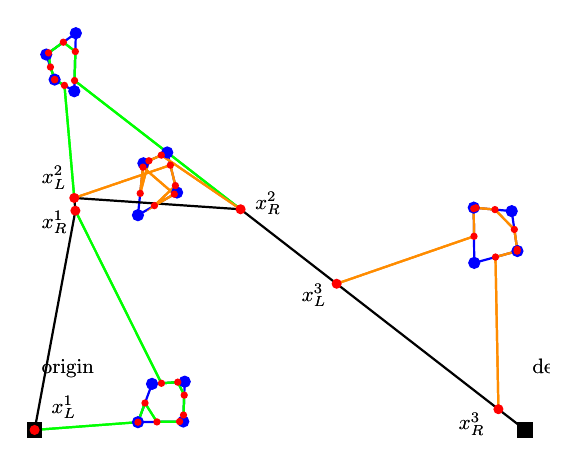
\begin{tikzpicture}
\definecolor{color0}{rgb}{1,0.549019607843137,0}
\begin{axis}[
hide x axis,
hide y axis,
scaled x ticks=manual:{}{\pgfmathparse{#1}},
scaled y ticks=manual:{}{\pgfmathparse{#1}},
tick align=outside,
x grid style={white!69.0196078431373!black},
xmajorticks=false,
xmin=-5, xmax=105,
xtick style={color=black},
xticklabels={},
y grid style={white!69.0196078431373!black},
ymajorticks=false,
ymin=-5, ymax=75,
ytick style={color=black},
yticklabels={}
]
\path [draw=blue, thick]
(axis cs:21.0696182692914,1.38670279952717)
--(axis cs:30.306045132353,1.50447958089156);

\path [draw=blue, thick]
(axis cs:21.0696182692914,1.38670279952717)
--(axis cs:23.9355243392435,8.22107815581281);

\path [draw=blue, thick]
(axis cs:30.306045132353,1.50447958089156)
--(axis cs:30.6007400849981,8.61180925900065);

\path [draw=blue, thick]
(axis cs:23.9355243392435,8.22107815581281)
--(axis cs:30.6007400849981,8.61180925900065);

\path [draw=blue, thick]
(axis cs:4.08370396767994,62.5193171258523)
--(axis cs:8.09069545603466,60.4417973648425);

\path [draw=blue, thick]
(axis cs:4.08370396767994,62.5193171258523)
--(axis cs:2.37426610997379,66.9905560181573);

\path [draw=blue, thick]
(axis cs:8.09069545603466,60.4417973648425)
--(axis cs:8.40433589338944,70.7975020391092);

\path [draw=blue, thick]
(axis cs:2.37426610997379,66.9905560181573)
--(axis cs:8.40433589338944,70.7975020391092);

\path [draw=blue, thick]
(axis cs:21.0664581490033,38.3255279820558)
--(axis cs:29.0472438012912,42.369596955967);

\path [draw=blue, thick]
(axis cs:21.0664581490033,38.3255279820558)
--(axis cs:22.1750046919912,47.5858849832036);

\path [draw=blue, thick]
(axis cs:29.0472438012912,42.369596955967)
--(axis cs:27.0356718607916,49.5164362980235);

\path [draw=blue, thick]
(axis cs:22.1750046919912,47.5858849832036)
--(axis cs:27.0356718607916,49.5164362980235);

\path [draw=blue, thick]
(axis cs:89.6170857784204,29.8130206242151)
--(axis cs:98.4204942730176,31.9280359170996);

\path [draw=blue, thick]
(axis cs:89.6170857784204,29.8130206242151)
--(axis cs:89.5168058385155,39.6742972814671);

\path [draw=blue, thick]
(axis cs:98.4204942730176,31.9280359170996)
--(axis cs:97.2556927544101,39.0446066906692);

\path [draw=blue, thick]
(axis cs:89.5168058385155,39.6742972814671)
--(axis cs:97.2556927544101,39.0446066906692);

\path [draw=black, thick]
(axis cs:0,0)
--(axis cs:5.19517108668237e-05,5.19721988422751e-05)
--(axis cs:8.31804668177588,39.1256215879103)
--(axis cs:8.0902667404291,41.3992381927182)
--(axis cs:41.9928361091472,39.3784823234059)
--(axis cs:61.5718673452208,26.0879192386296)
--(axis cs:94.5456634712005,3.70413789044963)
--(axis cs:100,0);
\path [draw=green, thick]
(axis cs:5.19517108668237e-05,5.19721988422751e-05)
--(axis cs:21.0696185355958,1.3867034345879)
--(axis cs:22.5025656416375,4.80387697389931)
--(axis cs:24.9379489929542,1.43602918392242)
--(axis cs:29.5561397992636,1.49491728610282)
--(axis cs:30.353931133669,2.65937414309857)
--(axis cs:30.5012780269027,6.21302491945877)
--(axis cs:29.1826401424249,8.52867680295897)
--(axis cs:25.850065249296,8.33331318471784)
--(axis cs:8.31804668177588,39.1256215879103);
\path [draw=green, thick]
(axis cs:5.19517108668237e-05,5.19721988422751e-05)
--(axis cs:21.0696185355958,1.3867034345879)
--(axis cs:22.5025656416375,4.80387697389931)
--(axis cs:24.9379489929542,1.43602918392242)
--(axis cs:29.5561397992636,1.49491728610282)
--(axis cs:30.353931133669,2.65937414309857)
--(axis cs:30.5012780269027,6.21302491945877)
--(axis cs:29.1826401424249,8.52867680295897)
--(axis cs:25.850065249296,8.33331318471784)
--(axis cs:8.31804668177588,39.1256215879103);
\path [draw=green, thick]
(axis cs:8.0902667404291,41.3992381927182)
--(axis cs:6.08717590107675,61.4805695906112)
--(axis cs:4.0837005407278,62.5193189026369)
--(axis cs:4.08369465698464,62.5193414790879)
--(axis cs:3.22897670117108,64.7549583801393)
--(axis cs:2.84174575638185,67.2856885528858)
--(axis cs:5.85674978390742,69.1891420779693)
--(axis cs:8.3052804744899,67.5269139951667)
--(axis cs:8.14846106263484,62.3490882974996)
--(axis cs:41.9928361091472,39.3784823234059);
\path [draw=color0, thick]
(axis cs:8.0902667404291,41.3992381927182)
--(axis cs:27.6728191506586,47.2527393224256)
--(axis cs:28.7000788954416,43.6030262742796)
--(axis cs:24.4315739690114,40.0307185577996)
--(axis cs:28.4696719165738,42.0769264544708)
--(axis cs:22.0922910532811,46.8949281369037)
--(axis cs:21.5323008920902,42.2169930131509)
--(axis cs:23.3011399504012,48.0331614224841)
--(axis cs:25.830886920397,49.0379219151249)
--(axis cs:41.9928361091472,39.3784823234059);
\path [draw=green, thick]
(axis cs:8.0902667404291,41.3992381927182)
--(axis cs:6.08717590107675,61.4805695906112)
--(axis cs:4.0837005407278,62.5193189026369)
--(axis cs:4.08369465698464,62.5193414790879)
--(axis cs:3.22897670117108,64.7549583801393)
--(axis cs:2.84174575638185,67.2856885528858)
--(axis cs:5.85674978390742,69.1891420779693)
--(axis cs:8.3052804744899,67.5269139951667)
--(axis cs:8.14846106263484,62.3490882974996)
--(axis cs:41.9928361091472,39.3784823234059);
\path [draw=color0, thick]
(axis cs:8.0902667404291,41.3992381927182)
--(axis cs:27.6728191506586,47.2527393224256)
--(axis cs:28.7000788954416,43.6030262742796)
--(axis cs:24.4315739690114,40.0307185577996)
--(axis cs:28.4696719165738,42.0769264544708)
--(axis cs:22.0922910532811,46.8949281369037)
--(axis cs:21.5323008920902,42.2169930131509)
--(axis cs:23.3011399504012,48.0331614224841)
--(axis cs:25.830886920397,49.0379219151249)
--(axis cs:41.9928361091472,39.3784823234059);
\path [draw=color0, thick]
(axis cs:61.5718673452208,26.0879192386296)
--(axis cs:89.5688132333832,34.5600210912317)
--(axis cs:89.5186458802408,39.4933522137777)
--(axis cs:89.9608257385526,39.6381686810341)
--(axis cs:93.8383627815696,39.3226648342931)
--(axis cs:97.7899505784608,35.7804594900926)
--(axis cs:98.374626227098,32.2082752452751)
--(axis cs:98.3537907014276,31.9120104112867)
--(axis cs:93.9472998319943,30.8533527808329)
--(axis cs:94.5456634712005,3.70413789044963);
\path [draw=color0, thick]
(axis cs:61.5718673452208,26.0879192386296)
--(axis cs:89.5688132333832,34.5600210912317)
--(axis cs:89.5186458802408,39.4933522137777)
--(axis cs:89.9608257385526,39.6381686810341)
--(axis cs:93.8383627815696,39.3226648342931)
--(axis cs:97.7899505784608,35.7804594900926)
--(axis cs:98.374626227098,32.2082752452751)
--(axis cs:98.3537907014276,31.9120104112867)
--(axis cs:93.9472998319943,30.8533527808329)
--(axis cs:94.5456634712005,3.70413789044963);
\addplot [draw=blue, fill=blue, mark=*, only marks]
table{%
x  y
21.0696182692914 1.38670279952717
30.306045132353 1.50447958089156
23.9355243392435 8.22107815581281
30.6007400849981 8.61180925900065
};
\addplot [draw=blue, fill=blue, mark=*, only marks]
table{%
x  y
4.08370396767994 62.5193171258523
8.09069545603466 60.4417973648425
2.37426610997379 66.9905560181573
8.40433589338944 70.7975020391092
};
\addplot [draw=blue, fill=blue, mark=*, only marks]
table{%
x  y
21.0664581490033 38.3255279820558
29.0472438012912 42.369596955967
22.1750046919912 47.5858849832036
27.0356718607916 49.5164362980235
};
\addplot [draw=blue, fill=blue, mark=*, only marks]
table{%
x  y
89.6170857784204 29.8130206242151
98.4204942730176 31.9280359170996
89.5168058385155 39.6742972814671
97.2556927544101 39.0446066906692
};
\addplot [semithick, red, mark=*, mark size=1, mark options={solid}, only marks]
table {%
24.9379489929542 1.43602918392242
29.5561397992636 1.49491728610282
21.0696185355958 1.3867034345879
22.5025656416375 4.80387697389931
30.353931133669 2.65937414309857
30.5012780269027 6.21302491945877
29.1826401424249 8.52867680295897
25.850065249296 8.33331318471784
6.08717590107675 61.4805695906112
4.0837005407278 62.5193189026369
4.08369465698464 62.5193414790879
3.22897670117108 64.7549583801393
8.3052804744899 67.5269139951667
8.14846106263484 62.3490882974996
2.84174575638185 67.2856885528858
5.85674978390742 69.1891420779693
24.4315739690114 40.0307185577996
28.4696719165738 42.0769264544708
22.0922910532811 46.8949281369037
21.5323008920902 42.2169930131509
27.6728191506586 47.2527393224256
28.7000788954416 43.6030262742796
23.3011399504012 48.0331614224841
25.830886920397 49.0379219151249
98.3537907014276 31.9120104112867
93.9472998319943 30.8533527808329
89.5688132333832 34.5600210912317
89.5186458802408 39.4933522137777
97.7899505784608 35.7804594900926
98.374626227098 32.2082752452751
89.9608257385526 39.6381686810341
93.8383627815696 39.3226648342931
};

\addplot [semithick, black, opacity=1, mark=square*, mark size=2.5, mark options={solid}, only marks]
table {%
0 0
100 0
};
\addplot [semithick, red, opacity=1, mark=*, mark size=1.5, mark options={solid}, only marks]
table {%
5.19517108668237e-05 5.19721988422751e-05
8.31804668177588 39.1256215879103
8.0902667404291044 41.399238192718173
41.9928361091472 39.3784823234059
61.571867345220838 26.087919238629631
94.5456634712005 3.70413789044963
};
\draw (0, 10) node[
  scale=0.75,
  anchor=base west,
  text=black,
  rotate=0.0
]{origin};
\draw (axis cs:2,3) node[
  scale=0.75,
  anchor=base west,
  text=black,
  rotate=0.0
]{$x_L^1$};
\draw (axis cs:0,36) node[
  scale=0.75,
  anchor=base west,
  text=black,
  rotate=0.0
]{$x_R^1$};
\draw (axis cs:0,44) node[
  scale=0.75,
  anchor=base west,
  text=black,
  rotate=0.0
]{$x_L^2$};
\draw (axis cs:43.4928361091472,39.3784823234059) node[
  scale=0.75,
  anchor=base west,
  text=black,
  rotate=0.0
]{$x_R^2$};
\draw (axis cs:53,23) node[
  scale=0.75,
  anchor=base west,
  text=black,
  rotate=0.0
]{$x_L^3$};
\draw (axis cs:85,0) node[
  scale=0.75,
  anchor=base west,
  text=black,
  rotate=0.0
]{$x_R^3$};
\draw (100,10) node[
  scale=0.75,
  anchor=base west,
  text=black,
  rotate=0.0
]{dest};
\draw (0, 10) node[
  scale=0.75,
  anchor=base west,
  text=black,
  rotate=0.0
]{origin};
\draw (axis cs:2,3) node[
  scale=0.75,
  anchor=base west,
  text=black,
  rotate=0.0
]{$x_L^1$};
\draw (axis cs:0,36) node[
  scale=0.75,
  anchor=base west,
  text=black,
  rotate=0.0
]{$x_R^1$};
\draw (axis cs:0,44) node[
  scale=0.75,
  anchor=base west,
  text=black,
  rotate=0.0
]{$x_L^2$};
\draw (axis cs:43.4928361091472,39.3784823234059) node[
  scale=0.75,
  anchor=base west,
  text=black,
  rotate=0.0
]{$x_R^2$};
\draw (axis cs:53,23) node[
  scale=0.75,
  anchor=base west,
  text=black,
  rotate=0.0
]{$x_L^3$};
\draw (axis cs:85,0) node[
  scale=0.75,
  anchor=base west,
  text=black,
  rotate=0.0
]{$x_R^3$};
\draw (100,10) node[
  scale=0.75,
  anchor=base west,
  text=black,
  rotate=0.0
]{dest};
\end{axis}
\end{tikzpicture}
\subcaption{[b]}
\caption{Example of feasible solution [a] and optimal solution [b] for a problem instance with 4 graphs and 2 drones.}
\label{fig:illustrative}
\end{figure}